\subsubsection{UC9 - Visualizzazione address utente}
\begin{figure}[h]
	\centering
	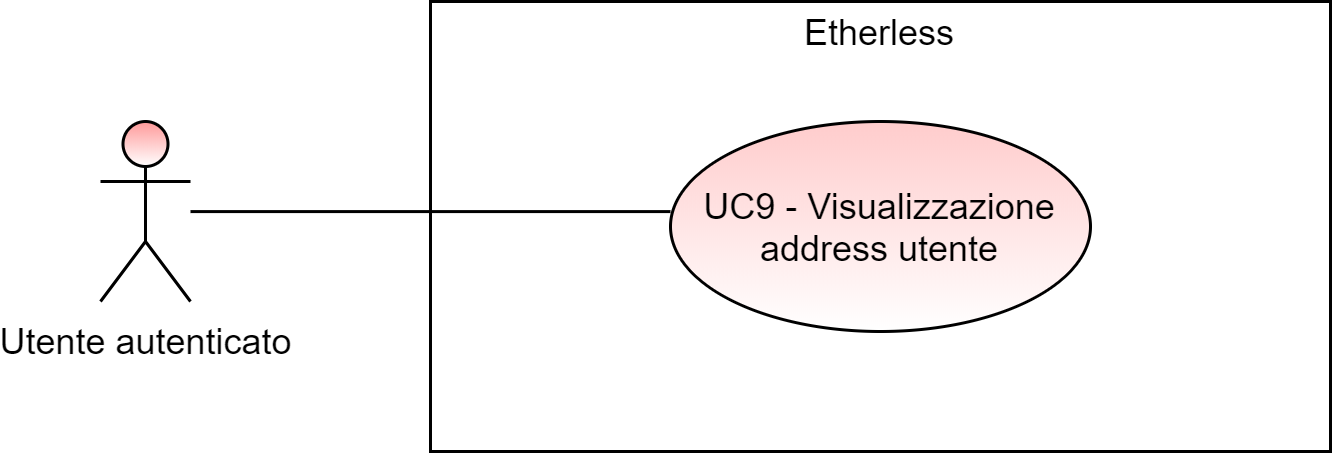
\includegraphics[scale=\ucs]{./res/img/UC9G.png}
	\caption {UC9 - Visualizzazione address utente: schema generale}
\end{figure}
\begin{itemize}
	\item \textbf{Attori primari:} \ua{};
	\item \textbf{Descrizione:} l’utente richiede la visualizzazione del campo address associato al proprio account eseguendo il comando \whoami{}. Il sistema stampa a video tale informazione; 
	\item \textbf{Scenario principale:} 
		\begin{itemize}
			\item l'utente inserisce correttamente ed esegue il comando \whoami{}; 
			\item il sistema visualizza il campo address associato all’utente.
		\end{itemize}
	\item \textbf{Precondizione:} l’utente è stato autenticato correttamente e richiede di visualizzare l’indirizzo associato alla propria utenza;
	\item \textbf{Postcondizione:} la CLI riporta il campo address associato all’account dell’utente.
\end{itemize}